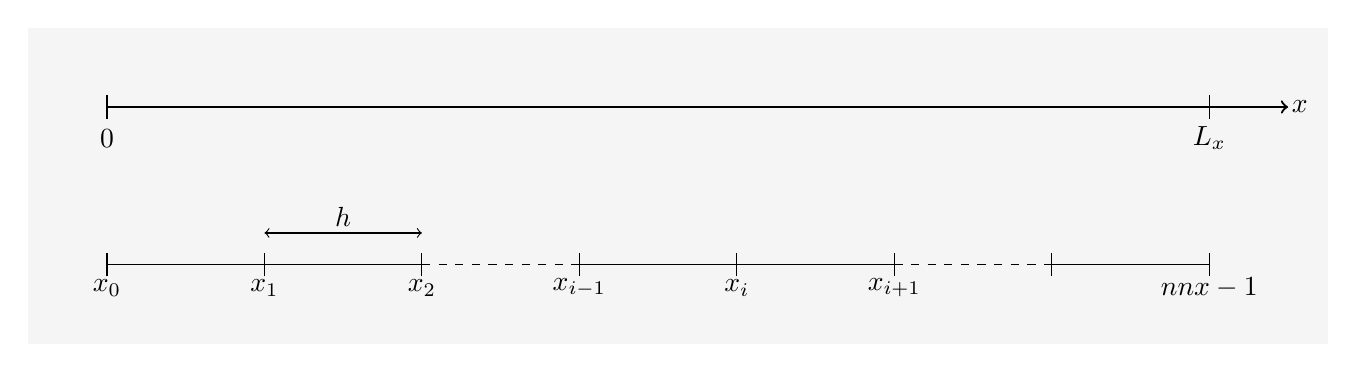
\begin{tikzpicture}
\draw[fill=gray!8,gray!8](0,0) rectangle (16.5,4);
%\draw[step=0.5cm,gray,very thin] (0,0) grid (16.5,4); %background grid
\node[] at (16.15,3) {$x$};
\node[] at (1,2.6) {$0$};
\node[] at (15,2.6) {$L_x$};
\draw[-] (1,2.85) -- (1,3.15) ; 
\draw[-] (15,2.85) -- (15,3.15) ; 
\draw[thick,->] (1,3) -- (16,3) ; 

%\draw[fill=gray!13,gray!13](1,1) rectangle (8,3);
%\draw[thick] (1,1) -- (5,1) -- (5,4) -- (1,4) -- cycle;  

\draw[-] (1,1) -- (5,1) ; 
\draw[dashed] (5,1) -- (7,1) ; 
\draw[-] (7,1) -- (11,1) ; 
\draw[dashed] (11,1) -- (13,1) ; 
\draw[-] (13,1) -- (15,1) ; 

\draw[-] (1,0.85) -- (1,1.15) ; 
\draw[-] (3,0.85) -- (3,1.15) ; 
\draw[-] (5,0.85) -- (5,1.15) ; 
\draw[-] (7,0.85) -- (7,1.15) ; 
\draw[-] (9,0.85) -- (9,1.15) ; 
\draw[-] (11,0.85) -- (11,1.15) ; 
\draw[-] (13,0.85) -- (13,1.15) ; 
\draw[-] (15,0.85) -- (15,1.15) ; 

\node[] at (7,0.7) {$x_{i-1}$};
\node[] at (9,0.7) {$x_i$};
\node[] at (11,0.7) {$x_{i+1}$};

\node[] at (1,0.7) {$x_0$};
\node[] at (3,0.7) {$x_1$};
\node[] at (5,0.7) {$x_2$};
\node[] at (15,0.7) {$nnx-1$};

\draw[<->] (3,1.4) -- (5,1.4) ; 
\node[] at (4,1.6) {$h$};

\end{tikzpicture}

